\section{The Birkhoff Diamond}
\label{sec:diamond}

\begin{figure}[!h]
    \centering
    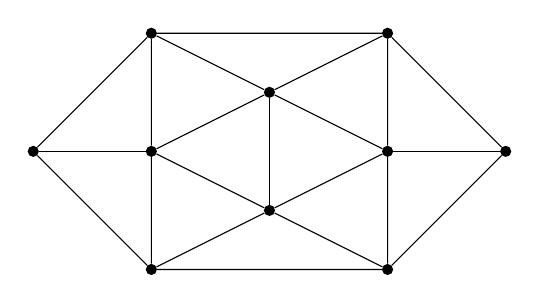
\begin{tikzpicture}[scale=1.5]
        \node[circle, fill, scale=0.015cm] (l1) at (-2, 0) { };
        \node[circle, fill, scale=0.015cm] (l2) at (-1, 1) { };
        \node[circle, fill, scale=0.015cm] (l3) at (-1, 0) {};
        \node[circle, fill, scale=0.015cm] (l4) at (-1, -1) {};

        \node[circle, fill, scale=0.015cm] (r1) at (2, 0) {};
        \node[circle, fill, scale=0.015cm] (r2) at (1, 1) {};
        \node[circle, fill, scale=0.015cm] (r3) at (1, 0) {};
        \node[circle, fill, scale=0.015cm] (r4) at (1, -1) {};

        \node[circle, fill, scale=0.015cm] (c1) at (0, 0.5) {};
        \node[circle, fill, scale=0.015cm] (c2) at (0, -0.5) {};

        \draw (l1) -- (l2) -- (r2) -- (r1) -- (r4) -- (l4) -- (l1);
        \draw (l1) -- (l3);
        \draw (l2) -- (l3) -- (l4);
        \draw (l2) -- (c1) -- (l3) -- (c2) -- (l4);
        \draw (c1) -- (c2);
        \draw (r2) -- (c1) -- (r3) -- (c2) -- (r4);
        \draw (r2) -- (r3) -- (r4);
        \draw (r1) -- (r3);
    \end{tikzpicture}
    \caption{The Birkhoff diamond with ring size 6}.
    \label{fig:diamond}
\end{figure}